\chapter{Crystallography and Point Defects}

\label{ch:crystallography}

\section{\zirconia\ phases and stabilisation}

\zirconia\ is unusual in exhibiting three commonly reported polytypes in its binary phase diagram (Figure \ref{figure:binary_phase_diagram}). Each will now be described and contrasted.

\begin{figure}[htp]
\centering
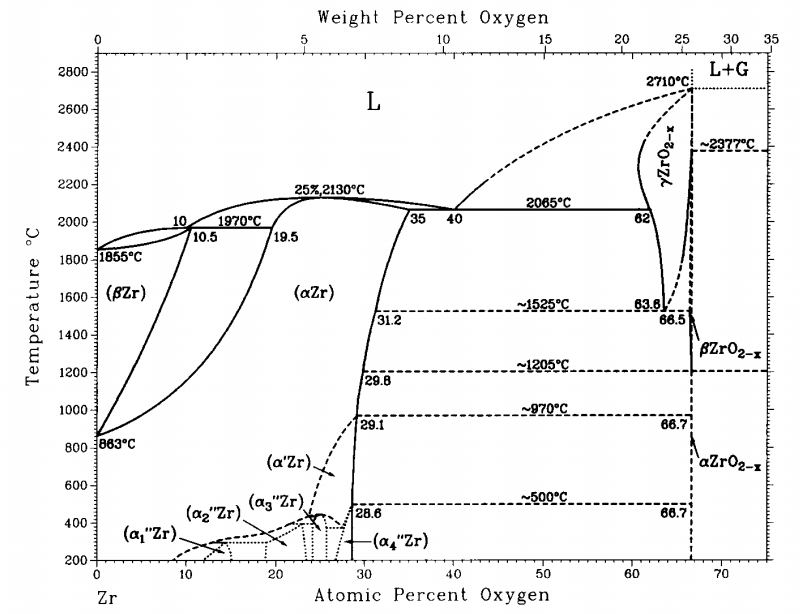
\includegraphics[height=9cm]{images/zro2_binary_phase.png}
\caption{Binary phase diagram of the Zr and O$_{2}$ system. Taken from \cite{Abriata1986TheSystem}.}
\label{figure:binary_phase_diagram}
\end{figure}

\subsection{Monoclinic}

A unit cell of monoclinic \zirconia\ is illustrated in Figure \ref{figure:coordination}. The dashed line (approximately 3.7\r{A} in length) shows the Zr-O bond which is broken when transitioning to monoclinic from the tetragonal phase.

\begin{figure}[htp] % Mono coordination figure
\centering
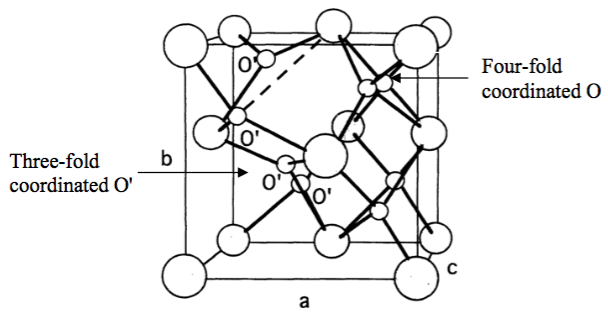
\includegraphics[height=6.2cm]{images/coordination.png}
\caption{A monoclinic zirconia unit cell indicating the two different oxygen bond coordinations. Small spheres represent oxygen ions while large spheres represent zirconium ions. Taken from \cite{Xia2010}.
\label{figure:coordination}}
\end{figure}

\begin{figure}[htp] % Mono Zr centre
\centering
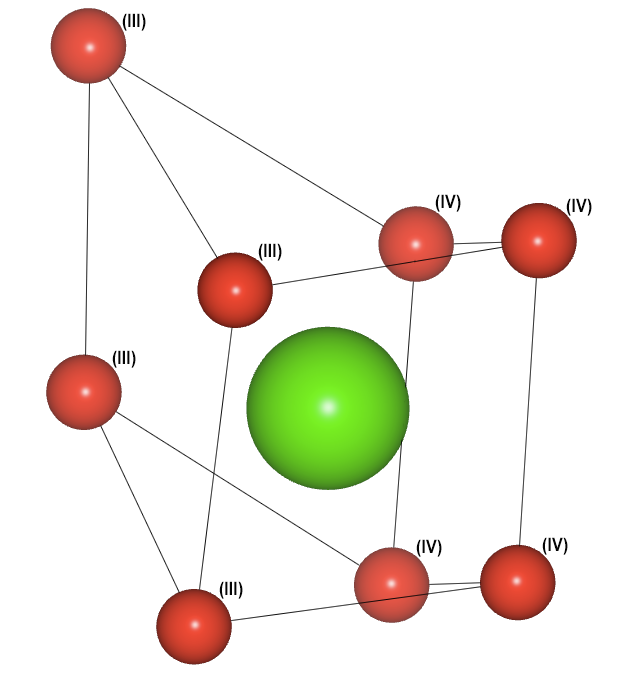
\includegraphics[height=6cm]{images/zr_centre_mono.png}
\caption{Zirconium centre in monoclinic \zirconia\ showing nearest oxygen atoms and their respective bond co-ordinations. Zirconium atoms are shown in green and oxygen atoms in red.}
\label{figure:monoschottky}
\end{figure}

\subsection{Common and predicted crystal structures}

Three common crystal structure at atmospheric conditions, as shown in table \ref{table:phases}.

\begin{table}[htp]
\centering
\onehalfspacing
\caption{\zirconia\ crystal structures and their stable temperatures at 1 atm \cite{Howard1988}.}
\label{table:phases}
\begin{tabular}{ccc}
\hline
{Crystal Structure} & {Space Group}    & {Temperature Range (K)} \\ \hline
\multicolumn{1}{c}{Monoclinic} & \multicolumn{1}{c}{$P2_1/c$} & \multicolumn{1}{c}{$T$ \textless\ 1440}     \\
\multicolumn{1}{c}{Tetragonal} & \multicolumn{1}{c}{$P4_2/nmc$} & \multicolumn{1}{c}{1440 \textless\ $T$ \textless\ 2640}        \\
\multicolumn{1}{c}{Cubic} & \multicolumn{1}{c}{$Fm\overline{3}m$}     & \multicolumn{1}{c}{2640 \textless\ $T$ \textless\ 2950}      \\ \hline
\end{tabular}
\end{table}

\subsubsection*{Volume expansion}

The phase transitions in \zirconia\ are accompanied by a change in volume, where the monoclinic phase is the least dense and the cubic phase is the most dense (see Figure \ref{figure:zrobonddistance}). This is especially significant in the case of the martensitic t-\zirconia\ to m-\zirconia\ transition, where the volume increases by around 9\% \cite{Gupta1977}. This has substantial implications for the creation and opening of cracks as \zirconia\ is a ceramic material with low toughness. This is especially relevant in a reactor scenario where temperature cycling (shutdown/startup or load-following behaviour) may lead to fatigue if the phase transition threshold is passed.

Another consequence of this large volume expansion is that a significant hysteresis effect is observed in the monoclinic/tetragonal phase transition, as shown in Figure \ref{fig:phasediagram}. 
%as the resulting coherency strain is likely to result in reduced mobility of fission products that have been embedded in the bulk crystal. 

\begin{figure}[htp]
  \centering
      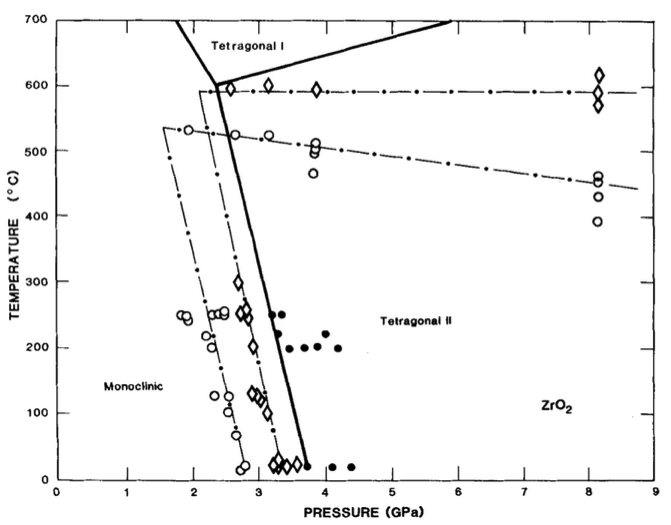
\includegraphics[height=10cm]{images/zirconiaphasediagram.png}
  \caption{Pressure-temperature phase diagram for \zirconia . Dash-dotted lines represent more recent data. Diamonds mark transition points during an increase in pressure/temperature, while open circles are used for a decrease in pressure/temperature. Solid circles represent transition points for a fresh, single crystal sample. Taken from \cite{gando2011partial}. \label{fig:phasediagram}}
\end{figure}

\begin{figure}
\begin{center}
\begin{tikzpicture}
	\begin{axis}
		[width=12cm, xlabel={Nearest neighbour Zr-O bond distance (\r{A})}, ylabel={Relative occurrence}, ymin=0, ymax=140, xmin=2.0, xmax=2.50, legend style={{draw=}, at={(0.95,0.95)}, anchor=north east, legend columns=1}]
		\addplot[no marks] table [x=zr_o_dist, y=monoclinic,]{dat/zr_o_bond_distances.dat}; \addlegendentry{Monoclinic};
        \addplot[no marks, dashed] table [x=zr_o_dist, y=tetragonal, ]{dat/zr_o_bond_distances.dat}; \addlegendentry{Tetragonal};
        \addplot[no marks, densely dotted] table [x=zr_o_dist, y=cubic,]{dat/zr_o_bond_distances.dat}; \addlegendentry{Cubic};
			\end{axis}
		\end{tikzpicture}
		\caption{Density plot of the nearest neighbour Zr-O bond distances in \zirconia\ for each crystal structure. Specific volumes from DFT simulations are 11.99, 11.51, and 11.13 \r{A}\textsuperscript{3}ion\textsuperscript{-1} for monoclinic, tetragonal, and cubic phases respectively.}
		\label{figure:zrobonddistance}
	\end{center}
\end{figure}


\subsection{Pressure stabilisation (isochoric + autostabilisation)}

The tetragonal and cubic phases of \zirconia\ are stabilised at high pressure. Since the oxide has a larger volume than the underlying metal (pilling-bedworth ratio of 1.5X), the growth of the oxide will itself impose stresses which may stabilise the tetragonal phase.

\subsection{Dopant stabilisation (lower valence cations)}

Some dopants will also stabilise the tetragonal and cubic phases of \zirconia. The most famous of which is yttrium, which at concentrations of 15\% (atomic), fully stabilises the cubic phase. Zirconia stabilised this way is known as YSZ. The way this works is by yttrium promoting the creation of oxygen vacancy defects (see equation XXX). This works in a similar way with several other lower valence cation dopants such as scandium and magnesium.

\section{Defect energies and defect volumes}

\subsection{Kr\"{o}ger-Vink notation}

Kr\"{o}ger-Vink notation \cite{kroger1956relations} is used throughout this work to describe defects. It is widely used in physical chemistry and is a useful shorthand for describing chemical reactions where we must consider conservation of mass, charge and also lattice sites. The notation syntax is of the form \ch{x^{y}_{z}}, where x is the atom or vacancy, y is the charge of the defect and z is the site the defect occupies. Positive and negative charges are indicated with dots (\ch{^{*}}) and dashes (\ch{^{'}}) respectively, otherwise a cross (\ch{^{x}}) is used to denote a neutral defect. The site may be either a lattice site (such as Zr or O in \zirconia ) or an interstitial site ($i$). Table \ref{table:krogervink} shows examples of several different types of defects and their respective Kr\"{o}ger-Vink notation.

\begin{table}[htp] % Kroger-Vink notation table
\onehalfspacing
\centering
\caption{Examples of Kr\"{o}ger-Vink notation for several defects in \zirconia .}
\label{table:krogervink}
\begin{tabular}{cc}
\hline
Defect & Kr\"{o}ger-Vink Notation \\ \hline
Anion vacancy & \ch{V_{O}^{**}} \\
Cation vacancy & \ch{V_{Zr}^{''''}} \\
Anion interstitial & \ch{O_{i}^{''}} \\
Cation interstitial & \ch{Zr_{i}^{****}} \\
Iodine on anion site & \ch{I_{O}^{*}} \\ \hline
\end{tabular}
\end{table}

\subsection{Incorporation and defect formation energies}

\subsubsection*{Isolated Frenkel defects}

Zr and O Frenkel defect formation energies were calculated via point defect DFT energies for the three structures. The formation energies of the isolated Frenkel defect pairs were defined as:
% Interstitial iodine defects were simulated in the neutral charge state at different interstitial sites in each phase. The incorporation energy of these defects, assuming a perfect lattice, was calculated using Equation \ref{equation_incorporation}:

\begin{equation}
\label{equation_frenkel}
E_{Frenkel} = E_{DFT}(V^{q}_{X}) + E_{DFT}(X^{-q}_{i}) - 2E_{DFT}(ZrO_2)% - \frac{E_{I_2}}{2}
\end{equation}

where $X$ is either Zr or O, $E_{DFT}(V^{q}_{X})$ is the energy of a supercell of \zirconia\ containing a single vacancy of charge $q$, $E_{DFT}(X^{-q}_{i})$ is the energy of a supercell of \zirconia\ containing a single interstitial with opposing charge $-q$, and $E_{DFT}(ZrO_2)$ is the energy of the non-defective supercell. Charges ranged from the fully charged case (+2 for oxygen vacancies, -4 for zirconium vacancies) to neutral. The interstitial sites, shown in Table \ref{table:interstitials}, were chosen based on standard vacant Wyckoff positions in each crystal structure \cite{theo1996international}.  In the case of oxygen vacancies in monoclinic \zirconia , a defect energy was obtained for both the (III) and (IV) co-ordinated oxygen sites, with the lowest energy value being used in the calculation of the Frenkel defect energy.

\begin{table}[htp] % Wyckoff positions of interstitials
\onehalfspacing
\centering
\caption{Wyckoff positions of interstitial sites used for each crystal structure.}
\label{table:interstitials}
\begin{tabular}{lcc}
\hline
\hspace{0.7 cm} {\bf Crystal Structure} \hspace{0.7 cm}                              & \hspace{0.7 cm} {\bf Interstitial Sites} \hspace{0.7 cm}                                               \\ \hline
\multicolumn{1}{c}{Monoclinic}              & $2a$, $2b$, $2c$, $2d$ \\
\multicolumn{1}{c}{Tetragonal}            & $2b$, $8e$                                   \\
\multicolumn{1}{c}{Cubic}       & $24d$, $4b$                                          \\ \hline
\end{tabular}
\end{table}

\subsubsection*{Isolated Schottky Defects}

Three Schottky energies were calculated for each structure, corresponding to fully charged, partially charged, and uncharged point defect energies. The Schottky formation energy was defined as:

\begin{equation}
\label{equation_schottky}
E_{Schottky} = E_{DFT}(V^{-2q}_{Zr}) + 2E_{DFT}(V^{q}_{O}) -\frac{3(n-1)}{n}E_{DFT}(ZrO_2)% - \frac{E_{I_2}}{2}
\end{equation}

where $n$ denotes the number of atoms in the supercell, $V^{q}_{O}$ denotes an oxygen vacancy with charge $q$, and $q$ varies from 2 to 0. This form maintains both the mass and charge balance of the Schottky defect description for \zirconia :

\begin{equation}
\label{generic_schottky}
Zr^{x}_{Zr} + 2O^{x}_{O} = V^{-2q}_{Zr} + 2V^{q}_{O} + ZrO_{2}
\end{equation}

This implies a rearrangement rather than complete removal of ions from the system. As with the Frenkel defects, the lowest energy vacancy energies were used to calculate Schottky formation energies. While there are multiple configurations of Schottky defects, such nuance cannot be accurately represented through a sum of individual vacancy defect energies. The values we present for Schottky defect formation energies should therefore be considered the lower bound for defect formation. 

\subsubsection*{Bound Frenkel Defects}

Bound Zr and O Frenkel defect formation energies in the three structures were calculated from DFT energies of supercells where a single ion was moved from its lattice site to an interstitial site. The formation energies of the bound Frenkel defect pairs were defined as:
% Interstitial iodine defects were simulated in the neutral charge state at different interstitial sites in each phase. The incorporation energy of these defects, assuming a perfect lattice, was calculated using Equation \ref{equation_incorporation}:

\begin{equation}
\label{equation_frenkel_bound}
E_{BoundFrenkel} = E_{DFT}(BoundFrenkel) - E_{DFT}(ZrO_2)% - \frac{E_{I_2}}{2}
\end{equation}

where $E_{DFT}(BoundFrenkel)$ is the energy of a supercell of \zirconia\ containing both a vacancy and interstitial defect of the same ion. The two defects were placed as far apart in the supercell as possible (7-8 \r{A}) to avoid recombination. The interstitial defect is assumed to fully compensate the charge of the vacancy defect, resulting in no overall charge on the supercell. The number and type of ions in the defective and non-defective supercell are the same, requiring no further steps to calculate the formation energy.
%Charges ranged from the fully charged case (+2 for oxygen, -4 for zirconium) to neutral. The interstitial sites, shown in Table \ref{table:interstitials}, were chosen based on standard vacant Wyckoff positions in each crystal structure \cite{theo1996international}.  In the case of oxygen vacancies in monoclinic \zirconia , a defect energy was obtained for both the (III) and (IV) co-ordinated oxygen sites. The lowest energies were used in the calculation of the Frenkel defect energy.

\subsubsection*{Bound Schottky Defects}


\begin{figure}[htp] % Tet Zr centre
\centering
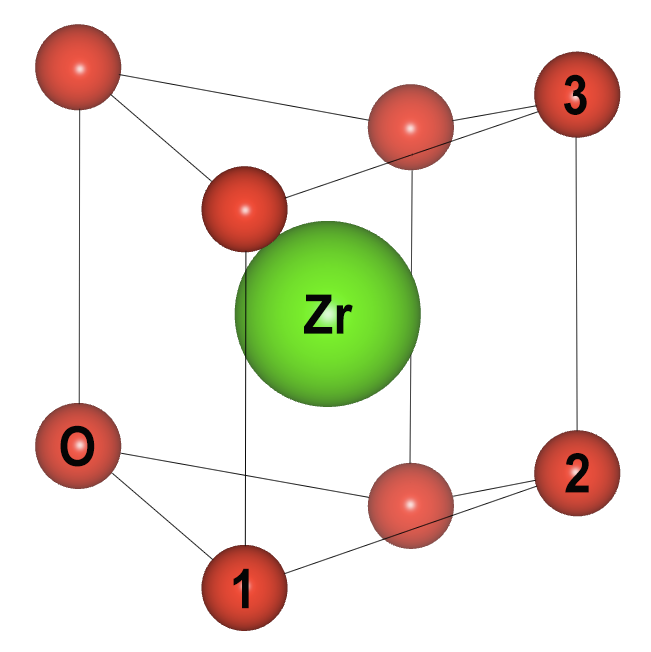
\includegraphics[height=6cm]{images/zr_centre_tet.png}
\caption{Zirconium centre showing nearest oxygen atoms in tetragonal \zirconia. Schottky trios indicated by oxygen enumeration. Zirconium atoms are shown in green and oxygen atoms in red.}
\label{figure:tetschottky}
\end{figure}

\begin{figure}[htp] % Cubic Zr centre
\centering
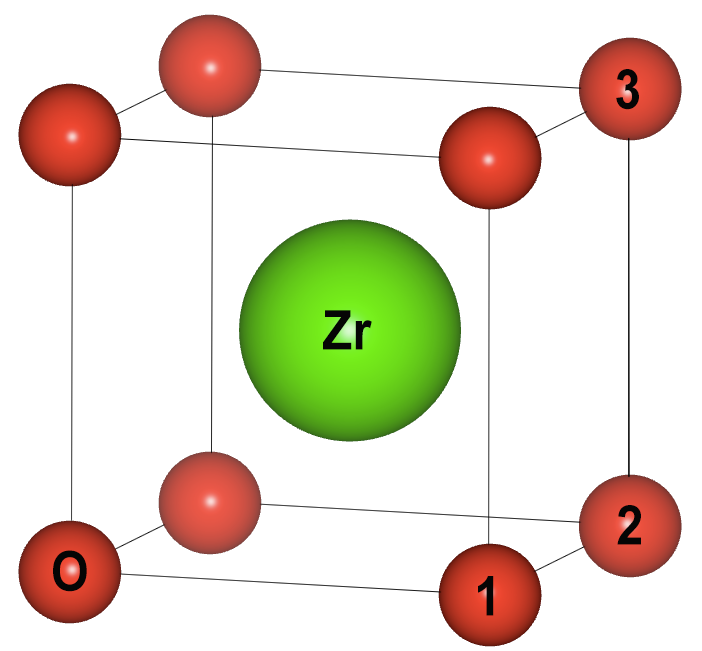
\includegraphics[height=6cm]{images/sd_cubic_zro2.png}
\caption{Zirconium centre showing nearest oxygen atoms in cubic \zirconia. Schottky trios indicated by oxygen enumeration. Zirconium atoms are shown in green and oxygen atoms in red.}
\label{figure:cubicschottky}
\end{figure}

Bound Schottky defects were modelled in a supercell of \zirconia\ by removing one Zr and two O atoms, in one of several possible nearest neighbour configurations as shown in Figures \ref{figure:monoschottky}, \ref{figure:tetschottky} and \ref{figure:cubicschottky}. Charge neutrality is maintained by the removal of a stoichiometric unit, therefore these defects were defined as neutral tri-vacancies (NTVs). The NTV formation energy was defined as:

\begin{equation}
\label{equation_NTV}
E_{NTV} = E_{DFT}(NTV) - \frac{n-3}{n}E_{DFT}(ZrO_2)% - \frac{E_{I_2}}{2}
\end{equation}

Where $E_{DFT}(NTV)$ is the energy of a supercell containing the NTV defect. As the defective supercell contains three fewer ions than the non-defective cell, the energy of the non-defective cell was adjusted by a proportional factor in our calculation. This form maintains both mass and charge balance of the Schottky defect description for \zirconia\ described in Equation \ref{generic_schottky}.

\section{Brouwer diagrams}

\subsection{Defect equilibria}

Typically in materials, several types of defects will exist simultaneously. These defects will be present at an equilibrium concentration based on their thermodynamic stability. There are several considerations to be made. For example, we expect a crystal lattice to be overall charge-neutral, otherwise we would see extreme behaviour at the macro scale which is not indicative of a low-energy state.

\subsection{Oxygen pressure dependence}

The equilibrium concentration of defects will be a function of the oxygen partial pressure, amongst other things like temperature and dopant concentrations. For materials in an equilibrium state, they are necessarily in equilibrium with their surroundings. This is why even metals in evacuated vacuum flasks will produce a metal vapour pressure. In the case of \zirconia\ in nuclear fuel cladding, we know that the ambient oxygen pressure will change over time. In particular, fission of UO$_{2}$ will result in the liberation of oxygen. This will result in an input of gaseous oxygen in the fuel cladding with increasing burn-up. The main oxygen sink is the Zr fuel cladding, into which the oxide grows. Other oxygen sinks include the oxidation of UO$_{2}$ to the ground state oxide U$_{3}$O$_{8}$, and oxidation of fission products. Oxidation of UO$_{2}$ is a slow process whose kinetics are largely independent of the oxygen partial pressure \cite{Desgranges2009NeutronUO2}, and will be slowed as free space in the cladding is reduced because it results in swelling of the fuel pellet. 

%\subsection{Brouwer diagram generation}